\chapter{Fundamentos teóricos}

Este capítulo tiene el propósito de presentar y describir los fundamentos teóricos que sustentan los métodos 
utilizados en el trabajo, además de justificar su importtancia para abordar los problemas planteados.

% --------------------------------------------------------------------------------------------------------------------
% MACHINE LEARNING ---------------------------------------------------------------------------------------------------
% --------------------------------------------------------------------------------------------------------------------

\section{Machine Learning}

Frente a la idea de intentar crear un programa que simulara directamente el comportamiento inteligente de una ``mente 
adulta'', Alan Turing ya vaticinó un enfoque alternativo \cite{turing1950}: que las máquinas pudieran aprender como 
lo hace un niño, mediante un ``proceso educativo'' con el cual se logra alcanzar progresivamente una ``mente adulta'', 
obteniendo así comportamientos inteligentes complejos.

% Athur Samuel años 50 surge machine learning
%He popularized the term "machine learning" in 1959.[4]
%Samuel, Arthur L. (1959). "Some Studies in Machine Learning Using the Game of Checkers". IBM Journal of Research and Development. 44: 206–226.

En las décadas de 1960, 1970 y 1980, en un contexto marcado por las limitaciones computacionales y el escepticismo 
académico surgió el \textit{machine learning} (ML) ---o \textit{aprendizaje automático}--- como una rama marginal de 
la IA, centrada en el desarrollo de modelos y algoritmos que permitiesen a las computadoras imitar la forma en la que 
los humanos aprenden, realizar tareas autónomas y mejorar su rendimiento a través de la experiencia y exposición a 
más datos. De esta forma, estos modelos podrían realizar predicciones o tomar decisiones sin ser programadas para 
cada caso.

Los años 90 y 2000 marcaron un punto de inflexión para el ML, gracias a los avances teóricos, el mayor poder 
computacional y la disponibilidad de grandes volúmenes de datos. De 2010 en adelante, la evolución del ML ha sido 
exponencial, marcada por la consolidación del \textit{deep learning}, la escalabilidad masiva y su integración en 
numerosas aplicaciones: de visión por computador, reconocimiento de lenguaje natural, robótica, diagnóstico médico 
y forense, finanzas o recomendación de contenidos, entre otros. De esta forma, el ML se ha convertido en un 
campo tan amplio y exitoso que ahora ``eclipsa'' al resto de campos de la IA \cite{domingos2015}.

El ML diferencia tres tipos de aprendizaje en base a tres tipos de retroalimentación \cite{rusell2009}: 

\begin{itemize}
    
    \item \textbf{Aprendizaje supervisado}, en el que el agente (refiriéndose con este al modelo de ML y su algoritmo 
    de aprendizaje) observa ejemplos de pares entrada-salida y aprende la función que mejor mapea las entradas 
    (inputs) a las salidas (outputs) correspondientes. El objetivo es generalizar este aprendizaje para hacer 
    predicciones precisas sobre datos nuevos y no vistos \cite{bishop2006}.

    \item \textbf{Aprendizaje por refuerzo}, en el que los datos de entrenamiento no contienen salida objetivo, sino 
    que contiene posibles resultados junto con medidas de calidad de dicho resultado, es decir, una función de 
    evaluación del estado. En este tipo de aprendizaje, el agente toma decisiones en un entorno y recibe recompensas 
    o penalizaciones por las acciones que realiza, ajustando su comportamiento mediante prueba y error, maximizando 
    la recompensa acumulada en el tiempo \cite{alpaydin2010}.

    \item \textbf{Aprendizaje no supervisado}, en el que el agente tampoco dispone de valores de salida, solo de 
    entrada \cite{bishop2006}, y los objetivos pueden ser muy variados, centrándose en descubrir patrones, 
    estructuras o relaciones ocultas en los datos. A diferencia de los otros enfoques, aquí no hay una ``respuesta 
    correcta'' predefinida, sino que el modelo debe inferir conocimiento directamente desde la distribución de los 
    datos.

\end{itemize}

Este trabajo se centrará en el aprendizaje supervisado, pues es este tipo de aprendizaje el empleado en los problemas
de clasificación y regresión que aplicaremos en el ámbito de la antropología forense.


% Retos en el aprendizaje supervisado


% No importa el formato de entrada



% --------------------------------------------------------------------------------------------------------------------

% En el \textbf{aprendizaje supervisado} \cite{bishop2006}, el agente (refiriéndose con este al 
% modelo de ML y su algoritmo de aprendizaje) observa ejemplos de pares entrada-salida y aprende
% la función que mejor mapea las entradas (inputs) a las salidas (outputs) correspondientes. El 
% objetivo es generalizar este aprendizaje para hacer predicciones precisas sobre datos nuevos y 
% no vistos.

% Hay dos principales tipos de problemas de aprendizaje supervisado: 

% \begin{itemize}
%     \item la \textit{clasificación} para cuando el valor de salida es una etiqueta categórica, y
%     \item la \textit{regresión} cuando el valor de salida es un valor continuo.
% \end{itemize}

% % --------------------------------------------------------------------------------------------------------------------

% En cambio, en el \textbf{aprendizaje por refuerzo}, los datos de entrenamiento no contienen 
% salida objetivo, sino que contiene posibles resultados junto con medidas de calidad de dicho 
% resultado, es decir, una función de evaluación del estado. En este tipo de aprendizaje, el 
% agente toma decisiones en un entorno y recibe recompensas o penalizaciones por las acciones 
% que realiza, ajustando su comportamiento mediante prueba y error, maximizando la recompensa 
% acumulada en el tiempo \cite{alpaydin2010}.  

% De esta forma, el algoritmo no aprende a dar una acción/salida a partir de un input, sino que 
% desarrolla una política que determina la mejor acción a tomar en cada estado del entorno, con 
% el objetivo de maximizar la recompensa acumulada a largo plazo.

% Esta aproximación es clave en aplicaciones como juegos, robótica, optimización de recursos y 
% sistemas conversacionales (ChatAI), donde las decisiones secuenciales y la interacción 
% dinámica con el entorno son fundamentales.

% % --------------------------------------------------------------------------------------------------------------------

% Y, por último, en el \textbf{aprendizaje no supervisado}, el agente tampoco dispone de valores 
% de salida, solo de entrada \cite{bishop2006}, y los objetivos pueden ser muy variados, 
% centrándose en descubrir patrones, estructuras o relaciones ocultas en los datos. 

% A diferencia de los otros enfoques, aquí no hay una "respuesta correcta" predefinida, sino que 
% el modelo debe inferir conocimiento directamente desde la distribución de los datos.

% Algunos problemas clásicos de este tipo de aprendizaje son: 

% \begin{itemize}

%     \item El \textit{clustering} o agrupamiento, donde el objetivo es encontrar clústeres o 
%     agrupaciones del input. Esto puede ser útil, por ejemplo, para una empresa que quiera 
%     segmentar sus clientes, o para identificar patrones en datos genéticos sin etiquetar.
    
%     \item La \textit{detección de anomalías} (\textit{outlier detection} en inglés), que 
%     consiste en encontrar instancias atípicas o inusuales en los datos. Sus aplicaciones 
%     incluyen: identificación de fraudes en transacciones bancarias, fallos en equipos 
%     industriales o identificación de ciberataques.

%     \item La \textit{reducción de dimensionalidad}, que trata de reducir el número de 
%     variables manteniendo la mayor información posible. Esto es útil para visualizar datos 
%     complejos o mejorar la eficiencia de algoritmos (p.ej., transformaciones PCA y t-SNE).

%     \item El \textit{aprendizaje de representaciones} (como los \textit{autoencoders}), 
%     donde el modelo busca capturar características latentes de los datos de manera eficiente. 
%     La compresión de archivos o la reducción de ruido en imágenes son algunos ejemplos de 
%     aplicaciones. 

% \end{itemize}



% --------------------------------------------------------------------------------------------------------------------

\subsection{Problemas de regresión}

Como se ha mencionado antes, la regresión es un tipo de problema clásico en el aprendizaje supervisado, y consiste 
en predecir el valor de una o más \textbf{variables continuas} objetivo a partir de unos datos de entrada 
\cite{bishop2006}, utilizando un modelo entrenado con ejemplos ya con valores conocidos.

Matemáticamente, este proceso implica modelar la relación entre la variable dependiente $Y$ y las variables
independientes $X$, de modo que se pueda predecir o explicar el comportamiento de $Y$ en función de los valores 
de $X$. El modelo aprende una función de predicción $f$ que, dado un nuevo ejemplo $i$ con características $X_i$, 
genera una estimación $\hat{Y_i}$:

$$
f(X_i) = f(X_{i0}, X_{i1}, \dots, X_{in}) = \hat{Y_i} = Y_i + \varepsilon_i
$$

donde 

\begin{itemize}
    \item $X_{i0},X_{i1}, \dots, X_{in}$ son las características o atributos del ejemplo $i$,
    \item $Y_i$ es el valor real de la variable objetivo para ese ejemplo,
    \item $\hat{Y_i}$ es la predicción generada por el modelo, y
    \item $\varepsilon_i$ representa el error o residuo \footnote{... a pesar de que en la literatura estos términos se distinguen, ...}, es decir, la diferencia entre la predicción y el valor real.
          Este término captura factores aleatorios o imprecisiones que el modelo no logra explicar perfectamente.
\end{itemize}

El análisis y la evaluación estadística del error son fundamentales para valorar la utilidad práctica del modelo y 
optimizar su capacidad predictiva mediante técnicas de ajuste y validación. Existen numerosas métricas para evaluar 
el rendimiento en problemas de regresión, pero tres destacan especialmente por ser \textit{model-agnostic}, es decir, 
aplicables a cualquier modelo de regresión independientemente del algoritmo subyacente. Estas son:

\begin{itemize}
    \item El \textbf{error absoluto medio (\textit{mean absolute error}, MAE)} mide el promedio de las diferencias 
    absolutas entre los valores reales ($Y_i$) y los valores predichos ($\hat{Y_i}$) por el modelo.

    $$
    MAE = \frac{1}{n} \sum_{i=1}^n{|Y_i - \hat{Y_i}|}
    $$

    donde $n$ es el número de ejemplos/instancias con las que se cuenta en los datos a evaluar.

    La interpretación más inmediata de esta métrica es que representa cuánto se desvía en promedio la 
    predicción del valor real sin considerar la dirección del error (positivo o negativo) y, por tanto, cuanto 
    más se acerque a cero el valor, mejor es el ajuste del modelo.

    Existe una variante denominada \textbf{error absoluto mediano (\textit{median absolute error}, MedAE)}, que 
    realiza la mediana de las diferencias absolutas, en vez de la media, aumentando la robustez frente a valores 
    atípicos con errores extremos.

    \item El \textbf{error cuadrático medio (\textit{mean squared error}, MSE)} mide el promedio de los errores al 
    cuadrado entre valores reales ($Y_i$) y los valores predichos ($\hat{Y_i}$) por el modelo.
    
    $$
    MSE = \frac{1}{n} \sum_{i=1}^n{(Y_i - \hat{Y_i})^2}
    $$

    Al igual que el MAE, cuantifica qué tan cerca están las predicciones de los valores reales, pero penaliza
    más los errores grandes, y es más sensible por tanto a valores atípicos.

    Como veremos más tarde, esta métrica es muy útil en optimización mediante gradiente descendente, usado 
    a la hora de entrenar modelos de regresión basados en redes neuronales.

    Y también tiene una variante, la \textbf{raíz del error cuadrático medio (\textit{root mean square error}, 
    RMSE)}, que se obtiene extrayendo la raíz cuadrada del MSE:

    $$
    RMSE = \sqrt{\frac{1}{n} \sum_{i=1}^{n}{(Y_i-\hat{Y_i})^2} }
    $$

    Esta métrica conserva las mismas unidades que la variable objetivo, lo que facilita su interpretación 
    práctica. Es comparable con el MAE en cuanto a escala, aunque sigue penalizando más los errores grandes.

    \item El \textbf{coeficiente de determinación}, o más conocido como \textbf{R² o bondad de ajuste}, mide la 
    proporción de la variabilidad de la variable dependiente ($Y$) que es explicada por el modelo.

    $$
    R^2 = 1 - \frac{\sum_{i=1}^n (Y_i - \hat{Y}_i)^2}{\sum_{i=1}^n (Y_i - \bar{Y})^2}
    $$

    donde 

    \begin{itemize}

        \item $Y_i$ es el valor real de la variable dependiente para la instancia $i$,
        
        \item $\hat{Y_i}$ es la predicción generada por el modelo, y
        
        \item $\bar{Y}$ es el promedio de los valores reales de la variable dependiente a lo largo de todas 
        las instancias del conjunto de datos.
    
    \end{itemize}
    

    El valor de esta métrica varía entre $-\infty$ y 1, y su interpretación es la siguiente:

    \begin{itemize}

        \item $R^2 \le 0$ significa que el modelo no explica ninguna variabilidad y que las predicciones del modelo 
        no son mejores que simplemente predecir la media de los valores reales.
        
        \item $R^2 \in \left(0,1\right)$ indica que el modelo está explicando una fracción de la variabilidad de los 
        datos, y cuanto más cercano sea a 1, mejor será el ajuste del modelo.
        
        \item $R^2 = 1$ indica un ajuste perfecto y, por tanto, el modelo explica toda la variabilidad de los datos. 
    
    \end{itemize}

    A diferencia de las anteriores, es una métrica relativa y adimensional, es decir, no depende de las unidades de 
    la variable objetivo y evalúa qué tan bien se ajusta el modelo en comparación con un modelo base que siempre 
    predice la media de los valores reales.
    
\end{itemize}

% Elementos visuales

No obstante, el uso exclusivo de métricas numéricas resulta en un análisis pobre, ya que estas no permiten 
identificar patrones ocultos, detectar relaciones no lineales ni distinguir entre errores positivos o 
negativos. Por esta razón, se recomienda completar el análisis con representaciones gráficas, tales como:

\begin{itemize}

    \item La \textbf{gráfica de puntos de valores reales vs. predichos}, que permite visualizar la relación entre las 
    predicciones del modelo y los valores reales. Idealmente, los puntos deberían alinearse alrededor de la recta 
    $Y=\hat{Y}$. Desviaciones sistemáticas indican sesgos o problemas de ajuste. Un ejemplo de esta gráfica lo 
    encontramos en la Figura \ref{fig:scatter_pred_vs_act_AE}.

    \begin{figure}[h]
        \centering
        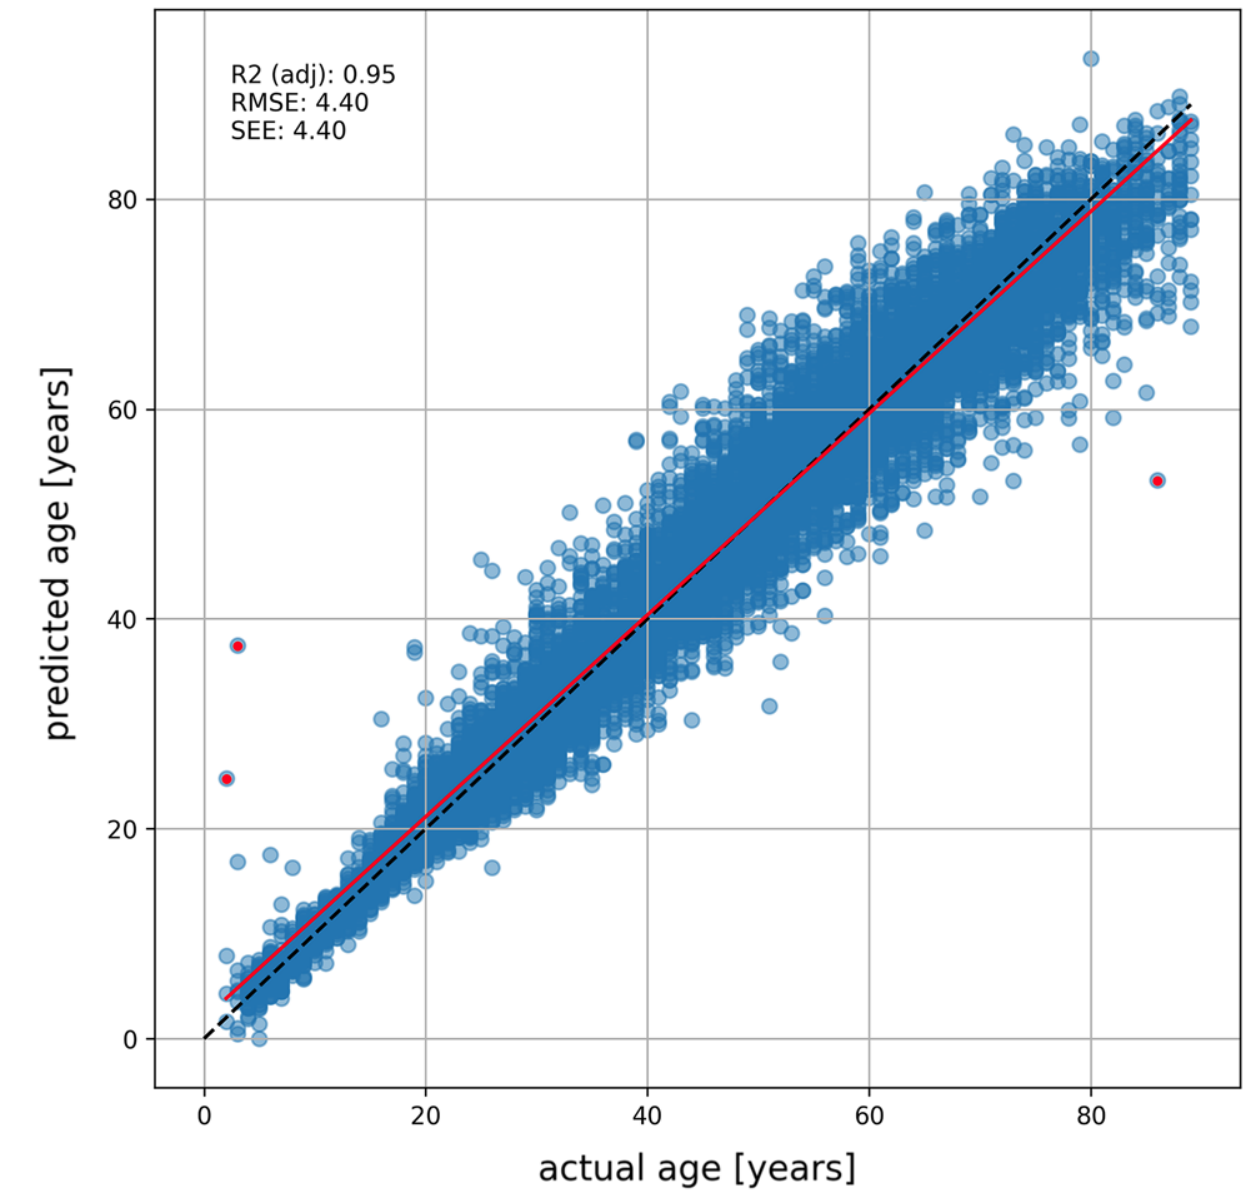
\includegraphics[width=0.5\textwidth]{capitulos/cap_02/imagenes/scatterplot_pred_vs_act_AE.png}
        \caption{Gráfica de puntos de valores de edad reales vs. predichos obtenidos por el modelo propuesto en 
        \cite{heinrich2024}. Se observan valores más dispersos en edades avanzadas.} 
        \label{fig:scatter_pred_vs_act_AE}
    \end{figure}

    \item También existe una versión más refinada de presentar esta información, especialmente útil en casos en los que 
    muchos datos sobrecargan la gráfica, en \textbf{la gráfica de cajas (en inglés \textit{boxplot}) de valores reales vs. 
    predichos}. Estos proporcionan una visión clara de la distribución de los datos, con mediana, cuartiles y valores 
    atípicos, ya sea agrupando por valores reales o por valores predichos.

    La Figura \ref{fig:boxplot_pred_vs_act_AE} muestra la distribución de las edades predichas en función de distintos 
    grupos de edad real, y viceversa, lo que facilita la identificación de errores en el desempeño del modelo.

    \begin{figure}[h]
        \centering
    
        \begin{subfigure}[b]{0.45\textwidth}
            \centering
            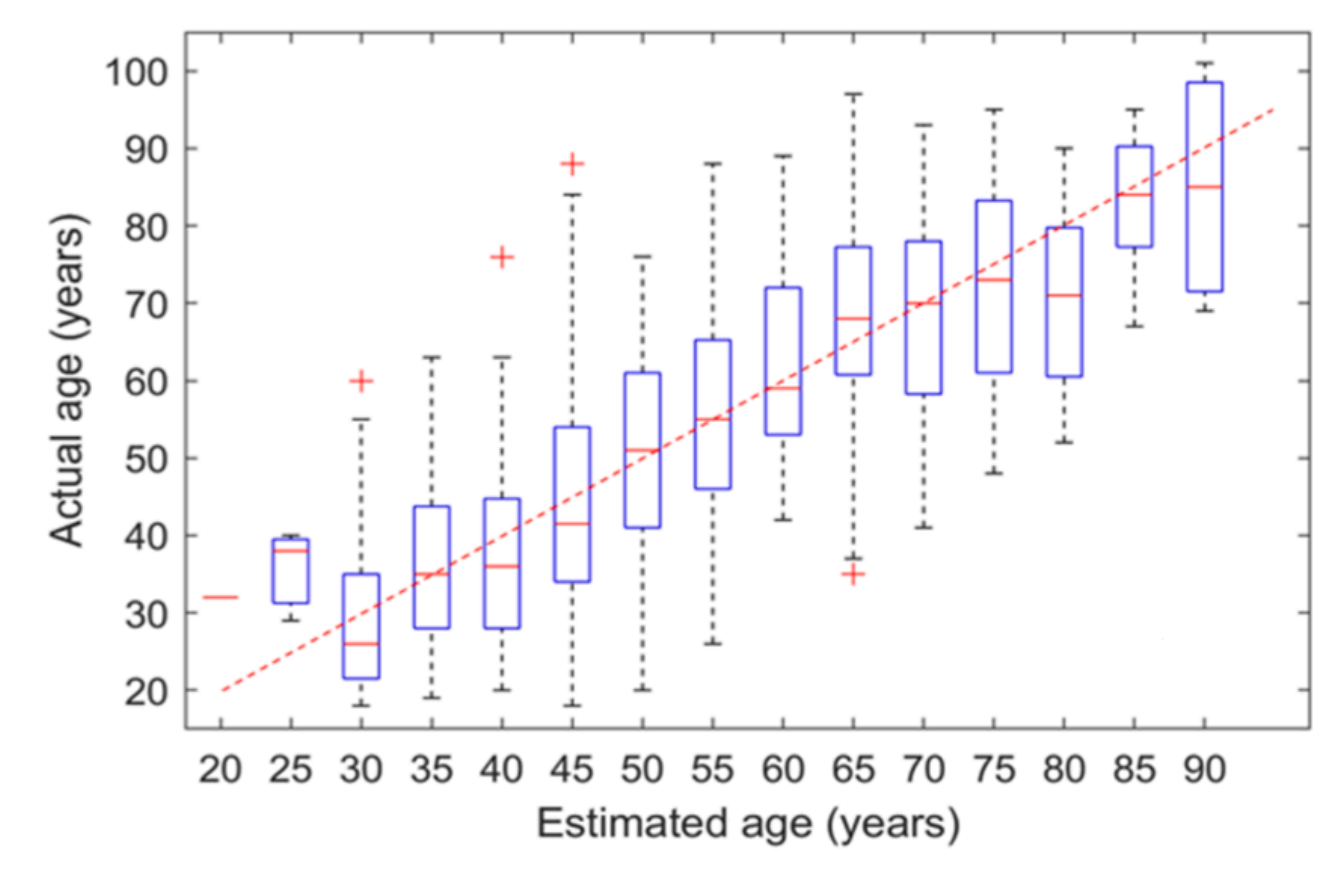
\includegraphics[width=\textwidth]{capitulos/cap_02/imagenes/boxplot_pred_vs_act_AE_1.png}
            \caption{Gráfica de cajas de edades reales en función de la estimada}
            \label{fig:boxplot_pred_vs_act_AE_a}
        \end{subfigure}
        \hfill
        \begin{subfigure}[b]{0.45\textwidth}
            \centering
            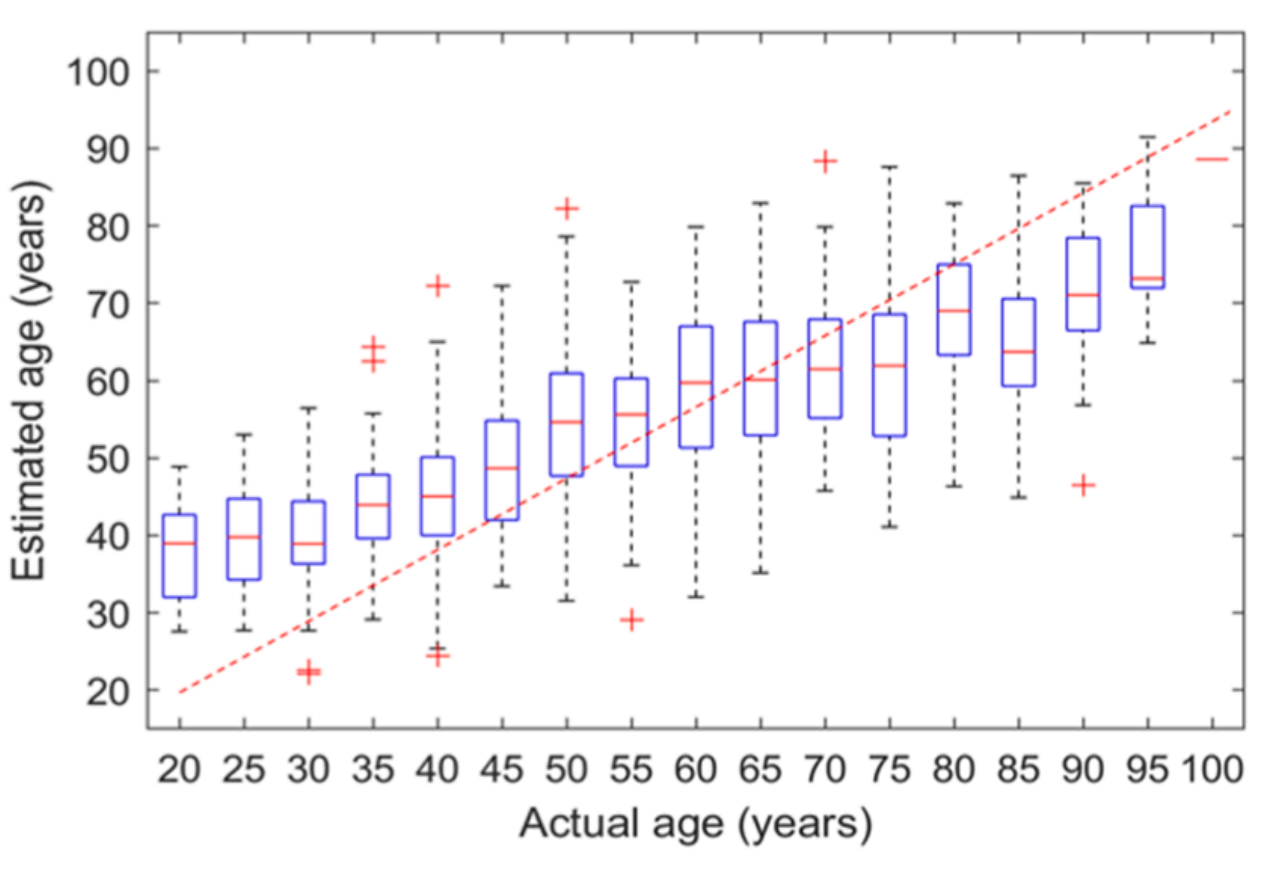
\includegraphics[width=\textwidth]{capitulos/cap_02/imagenes/boxplot_pred_vs_act_AE_2.png}
            \caption{Gráfica de cajas de edades estimadas en función de la real}
            \label{fig:boxplot_pred_vs_act_AE_b}
        \end{subfigure}
    
        \caption{Gráfica de cajas de valores de edad reales vs. predichos obtenidos por el modelo propuesto en \cite{stepanovsky2024}.
        Se observa en \ref{fig:boxplot_pred_vs_act_AE_a}, 
        y en \ref{fig:boxplot_pred_vs_act_AE_a} que se sobreestima la edad en personas jóvenes y se subestima en personas de edad avanzada.}
        \label{fig:boxplot_pred_vs_act_AE}
    \end{figure}

    \item El \textbf{histograma de residuos} muestra la distribución de los errores (\(Y_i - \hat{Y}_i\)) del 
    modelo. Una distribución simétrica y centrada en cero sugiere un buen ajuste, mientras que una distribución 
    sesgada o asimétrica podría indicar que el modelo está subajustado o que hay algún patrón no capturado por el 
    modelo. 

    Un ejemplo de este tipo de gráfica lo encontramos en la Figura \ref{fig:prob_dist_AEerror}, 
    donde se analizaba el error obtenido con el modelo propuesto en \cite{stepanovsky2024}.

    Histograma de errores residuales del modelo de regresión propuesto en \cite{verma2020} que predice la estatura 
    a partir de la longitud de la tibia.

    \begin{figure}[h]
        \centering
        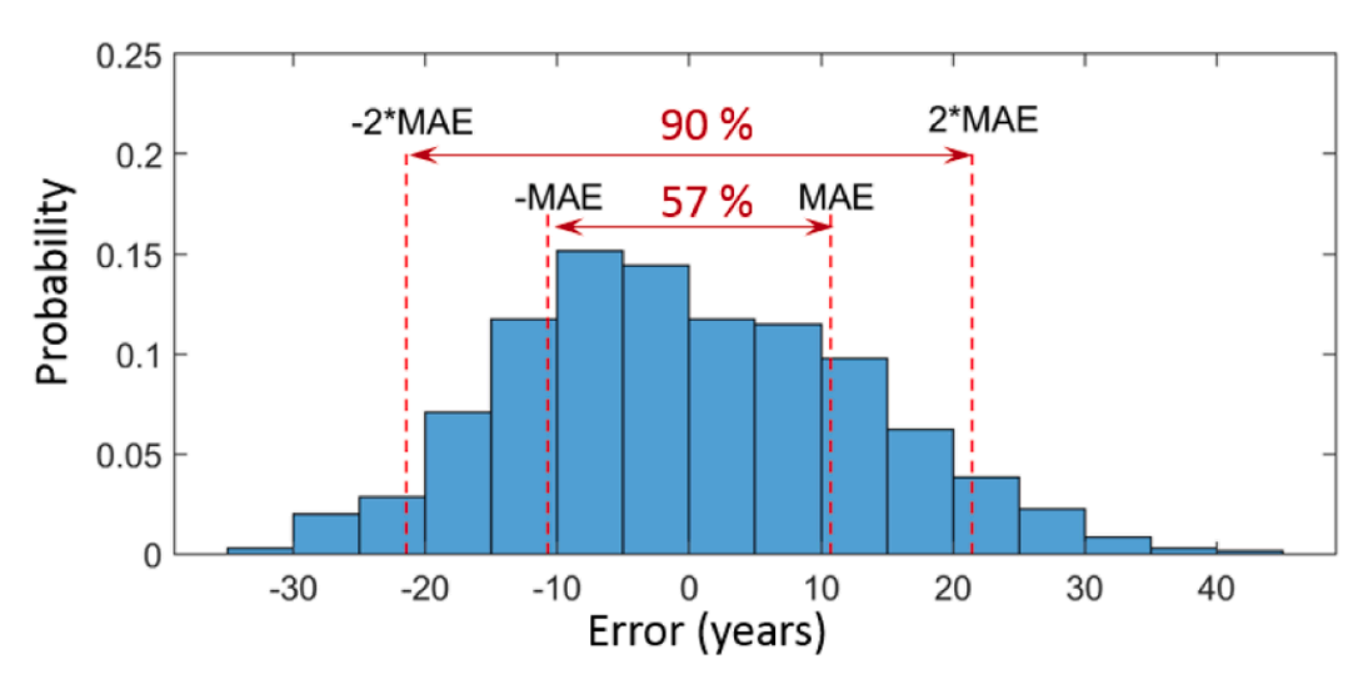
\includegraphics[width=0.8\textwidth]{capitulos/cap_02/imagenes/prob_distribution_AEerror.png}
        \caption{Histograma de errores residuales del modelo de estimación de edad propuesto en 
        \cite{stepanovsky2024}. Se evidencia una mayor probabilidad de errores negativos (infraestimaciones) 
        en comparación con los positivos Además, se destaca que el 57\% de las predicciones presentan un 
        error inferior al $\textnormal{MAE}$, y que el 90\% se encuentra dentro de un margen de error menor a 
        $2\textnormal{MAE}$.
        } 
        \label{fig:prob_dist_AEerror}
    \end{figure}


    \item Y una versión más completa que este último es la \textbf{gráfica de cajas de la distribución del error 
    en base a los valores reales o predichos}, que permite analizar cómo varía el error del modelo a lo largo de 
    diferentes rangos de valores, ya sean reales o predichos. Estas visualizaciones nos permiten detectar 
    fácilmente las fortalezas y debilidades en las predicciones del modelo, así como diagnosticar sesgo o 
    insuficiencia de datos en ciertas categorías.
    
    Un ejemplo ilustrativo de esta gráfica se presenta en la Figura \ref{fig:boxplot_error_vs_act_AE}, donde se 
    observa la variación del error del modelo propuesto en \cite{heinrich2024} a través de distintos rangos de edad real. 
    En particular, se evidencia una tendencia a cometer errores mayores en los grupos de edad más avanzada.

    \begin{figure}[h]
        \centering
        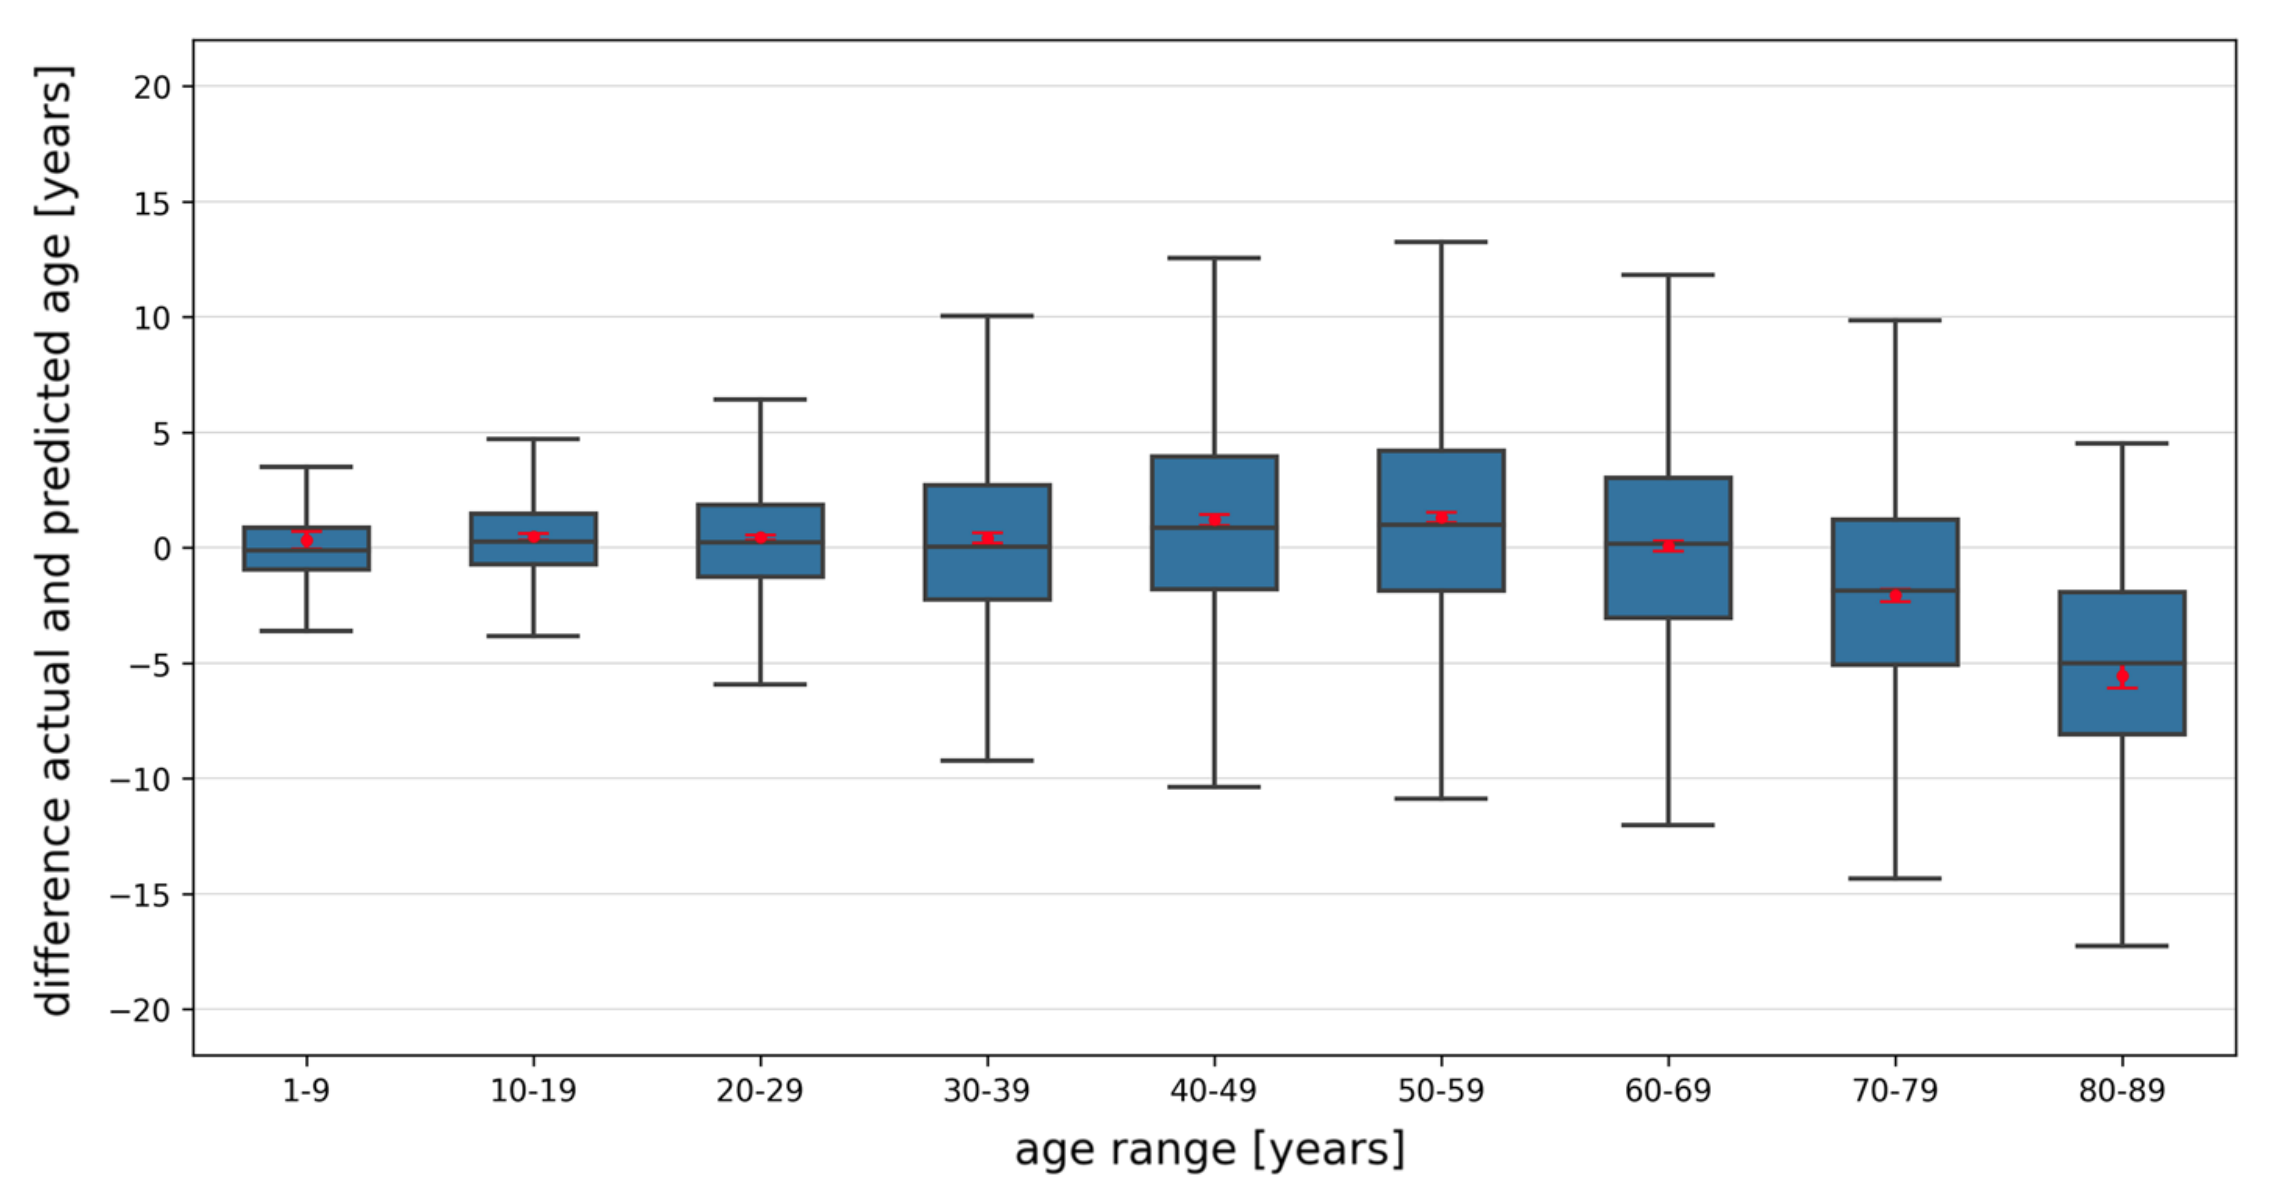
\includegraphics[width=0.95\textwidth]{capitulos/cap_02/imagenes/boxplot_error_vs_act_AE.png}
        \caption{Gráfica de cajas de la distribución del error de estimación de edad en función de la edad real, 
        obtenida en el modelo propuesto en \cite{heinrich2024}.} 
        \label{fig:boxplot_error_vs_act_AE}
    \end{figure}

\end{itemize}






% --------------------------------------------------------------------------------------------------------------------

\subsection{Problemas de clasificación}

En cambio, en los problemas de clasificación, los valores de salida son categóricos, denominados más comúnmente como
\textbf{clases}, y a cada valor individual asignado a una instancia de datos se le conoce como \textbf{etiqueta} 
(\textit{label} en inglés).

Existen multitud de variante de clasificación, que pueden diferenciarse según diversos criterios:

\begin{itemize}
    \item En base a la cardinalidad de las clases de salida: \textbf{clasificación binaria o multiclase}, según 
    si existen dos clases posibles o más de dos, respectivamente.

    \item En base al número de etiquetas asignadas a cada instancia: \textbf{clasificación con etiqueta única o 
    multietiqueta}, según si cada instancia pertenece a una sola clase o a varias de forma simultánea.

    \item En base a la certeza de la asignación de clases: \textbf{clasificación con etiqueta precisa o difusa}, 
    donde en el primer caso la asignación a una clase es determinista, y en el segundo caso se permite una 
    pertenencia parcial a varias clases con distintos grados de confianza o probabilidad.
    
\end{itemize}

No obstante, la mayoría de los problemas estudiados en la literatura corresponden a clasificación binaria o 
multiclase, con etiquetas únicas y asignación precisa \cite{bishop2006}, y son los que analizaremos en este
trabajo.

Se analizarán más a fondo los dos tipos de clasificación según su cardinalidad de clases, lo que tiene 
importantes implicaciones tanto en el diseño del modelo como en la evaluación de su desempeño: 

\begin{itemize}

    \item \textbf{Clasificación binaria}, que es aquella en la que existen únicamente dos clases posibles para la 
    variable objetivo, siendo común en problemas donde se desea discriminar entre dos estados mutuamente 
    excluyentes (p.ej., ``positivo'' vs. ``negativo'', ``spam'' vs. ``no spam'', ``fraude'' vs. ``no fraude'').
    
    Se suele denominar a una de las clases como ``positiva'' y a otra como ``negativa'' para facilitar la 
    interpretación de métricas como la precisión, la sensibilidad o la especifidad, si bien no tiene por qué 
    existir una connotación valorativa entre ambas clases.
    
    \item \textbf{Clasificación multiclase}: en este caso, la variable objetivo puede tomar más de dos valores 
    posibles, pertenecientes a un conjunto finito. Un ejemplo de problema clásico es el de clasificar dígitos
    manuscritos (0-9).

\end{itemize}


% Problemas comunes: clasificación desbalanceada

% Tanto en clasificación binaria como multiclase, un problema común es el desequilibrio de clases, donde una 
% clase tiene muchos más ejemplos que otra. Esto afecta el entrenamiento del modelo, ya que puede sesgarse hacia la 
% clase mayoritaria, ya que el modelo


Una vez definido los tipo de problemas de clasificación, es fundamental establecer cómo medir la efectividad del 
modelo predictivo. A continuación, se detallan los principales criterios y elementos gráficos utilizados para 
evaluar y comparar modelos de clasificación:

\begin{itemize}
    
    \item La \textbf{matriz de confusión} es una herramienta fundamental que permite visualizar el rendimiento de 
    modelos de clasificación, tanto binarios como multiclase.
    Esta muestra una tabla con tantas columnas y filas como clases haya. En un eje, se representan las 
    clases reales (etiquetas verdaderas), y en el otro eje, las clases predichas por el modelo.
    Cada celda de la matriz indica la cantidad de ejemplos que pertenecen a una clase real específica y que han 
    sido clasificados como una clase predicha específica (véase la Figura \ref{fig:conf_matrix_binary}).

    Idealmente, los valores se concentrarían en la diagonal principal, lo que indicaría que las predicciones 
    coinciden con los valores reales.

    \begin{figure}[h]
        \centering
        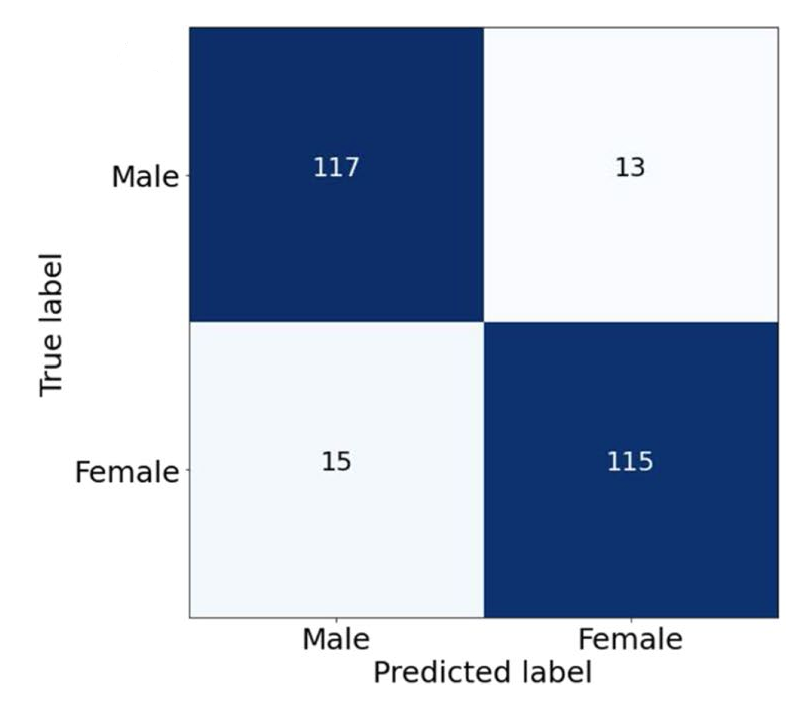
\includegraphics[width=0.6\textwidth]{capitulos/cap_02/imagenes/confusion_matrix_binary.png}
        \caption{Matriz de confusión para la estimación de sexo según el modelo \textit{random forest} propuesto 
                 en \cite{bidmos2023}.} 
        \label{fig:conf_matrix_binary}
    \end{figure}

    Esta visualización admite muchas variantes, por ejemplo en la Figura \ref{fig:conf_matrix_binary_relative}
    se representan los valores de cada celda en términos porcentuales de los ejemplos reales que hay de cada clase 
    ($< 18$ y $\ge 18$), lo que permite comparar la matriz de confusión general de todos los ejemplos 
    (\ref{fig:conf_matrix_general}) con la de ejemplos se sexo femenino (\ref{fig:conf_matrix_female}) y 
    sexo masculino (\ref{fig:conf_matrix_male}), permitiendo identificar posibles sesgos en el modelo respecto 
    al género, y así realizar una evaluación más precisa del rendimiento del modelo en diferentes subgrupos de
    la población.
    
    \begin{figure}[h]
        \centering
    
        \begin{subfigure}[b]{0.3\textwidth}
            \centering
            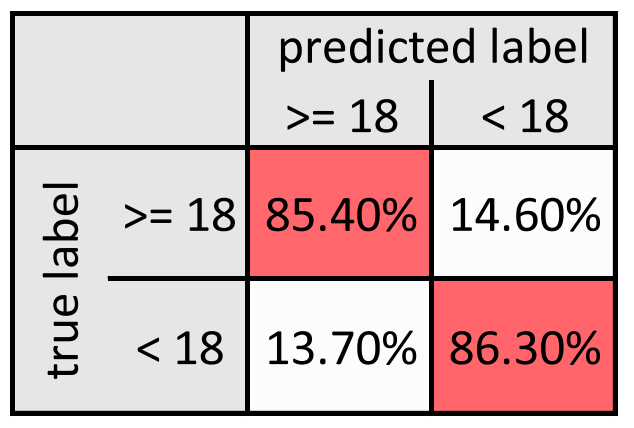
\includegraphics[width=\textwidth]{capitulos/cap_02/imagenes/confusion_matrix_binary_1.png}
            \caption{Sin información de sexo}
            \label{fig:conf_matrix_general}
        \end{subfigure}
        \hfill
        \begin{subfigure}[b]{0.3\textwidth}
            \centering
            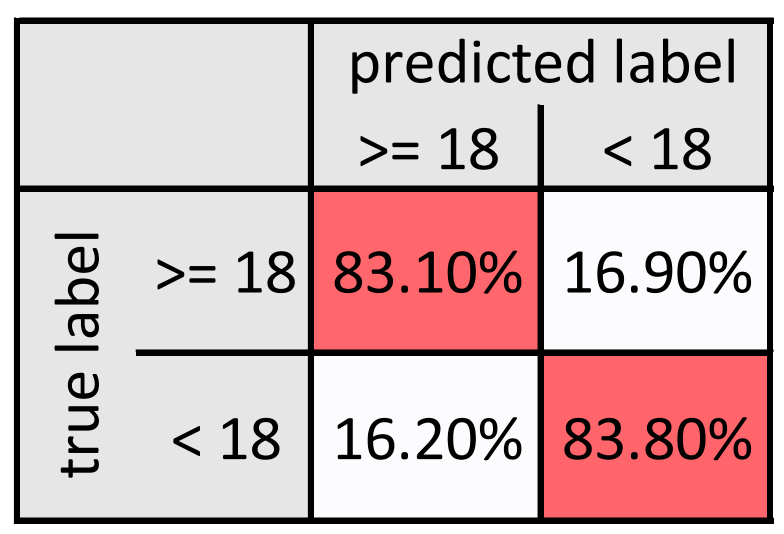
\includegraphics[width=\textwidth]{capitulos/cap_02/imagenes/confusion_matrix_binary_2.png}
            \caption{Sexo femenino}
            \label{fig:conf_matrix_female}
        \end{subfigure}
        \hfill
        \begin{subfigure}[b]{0.3\textwidth}
            \centering
            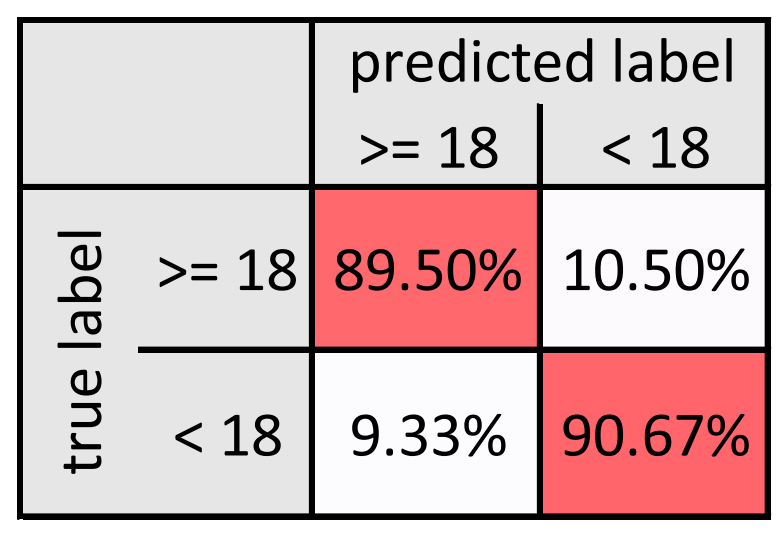
\includegraphics[width=\textwidth]{capitulos/cap_02/imagenes/confusion_matrix_binary_3.png}
            \caption{Sexo masculino}
            \label{fig:conf_matrix_male}
        \end{subfigure}
    
        \caption{Matrices de confusión para la estimación de mayoría/minoría de edad según el modelo de \cite{porto2020}.}
        \label{fig:conf_matrix_binary_relative}
    \end{figure}

    Prácticamente todas las métricas y visualizaciones parten de la información ofrecida en esta matriz. 
    

    \item La \textbf{exactitud (accuracy)} es la proporción de predicciones correctas sobre el total.
    
    $$
    \textnormal{Accuracy} = \frac{TP+TN}{TP+TN+FP+FN}
    $$

    Es la medida más intuitiva, si bien carece de utilidad en escenarios con clases desbalanceadas, ya que puede dar una 
    falsa impresión de buen desempeño si la clase mayoritaria domina la métrica. Es por esto que el análisis debe
    complementarse con otras métricas informativas.


    \item La \textbf{precisión (precision) y exhaustividad (recall)}
    
    $$
    \textnormal{Precision} = \frac{TP}{TP+FP}
    $$

    $$
    \textnormal{Recall} = \frac{TP}{TP+FN} = \textnormal{Sensitivity}
    $$
    

    \item El \textbf{F1-Score} 

    $$
    \textnormal{F1-Score} = 2 \cdot \frac{\textnormal{Precision} \cdot \textnormal{Recall}}{\textnormal{Precision} + \textnormal{Recall}}
    $$


    \item La \textbf{sensibilidad (sensitivity) y especifidad (specifity)}

    $$
    \textnormal{Sensitivity} = \frac{TP}{TP+FP}
    $$

    $$
    \textnormal{Specifity} = \frac{TN}{TN+FP}
    $$


\end{itemize}



% --------------------------------------------------------------------------------------------------------------------
% REDES NEURONALES ---------------------------------------------------------------------------------------------------
% --------------------------------------------------------------------------------------------------------------------

\section{Deep Learning}

El \textbf{aprendizaje profundo (\textit{deep learning}, DL)} es una familia de técnicas de ML que utiliza
redes neuronales de muchas capas. 
Las redes neuronales tienen su origen en el intento de modelar las redes de neuronas del cerebro 
\cite{mcculloch1943}. Se requirió de numerosas contribuciones teóricas ---como el perceptrón \cite{rosenblatt1958} 
o el algoritmo de \textit{backpropagation} \cite{rumelhart1986,werbos1994}, entre otras---, disponibilidad de datos 
estandarizados y un gran aumento en la capacidad computacional para poder escalar estar redes y obtener resultados 
sorprendentes en tareas complejas.

Las \textbf{redes neuronales profundas (\textit{deep neural networks}, DNNs)} destacan por su capacidad para 
aprender representaciones jerárquicas: cada capa extrae características progresivamente más abstractas 
\cite{lecun2015}, desde líneas en imágenes hasta formas geométricas complejas, objetos completos e incluso 
escenas compuestas.
Esta propiedad las hace excepcionalmente versátiles, ya que procesan datos de muy diversa naturaleza ---datos 
tabulares, imágenes, audio, texto y señales temporales---, dados que ellas mismas aprenden los procesos de 
extracción de características de estos, hasta ahora realizados ``a mano'' (mediante procesos diseñados por la 
ingeniería de características).

Gracias a ello, las DNNs han alcanzado rendimientos sobresalientes en dominios como visión artifical
(clasificación de imágenes, detección de objetos, segmentación) y procesamiento de lenguaje natural 
(traducción, generación de texto) \cite{redhat2024DeepLearningDefinition}.

No obstante, su eficacia depende críticamente de grandes volúmenes de datos y recursos computacionales,
lo que ha impulsado técnicas como el \textit{transfer learning} y modelos eficientes para democratizar 
su aplicación.


\subsection{El perceptrón multicapa}

El \textbf{perceptrón multicapa (\textit{multilayer perceptron}, MLP)}



\subsection{La red neuronal}



...

Así, una red neuronal está compuesta por: 

\begin{itemize}

    \item \textbf{una capa de entrada}, que debe coincidir con el formato de entrada de los datos, por ejemplo: el
    número de neuronas en la capa de entrada tiene que coincidir con el de características en problemas tabulares.
    No obstante, como veremos más tarde, en las CNNs no se requiere un tamaño fijo de imagen a la entrada.
    
    \item \textbf{una serie de capas ocultas}, donde se realizan las transformaciones no lineales de los datos. 
    Es en estas donde el diseño puede variar en número de neuronas y tipo de capas según la complejidad del 
    problema; y
    
    \item \textbf{una capa de salida}, que proporciona el resultado del modelo, su forma depende del problema a 
    resolver: en problemas de regresión, esta capa tendrá tantas neuronas como variables a predecir; en problemas de 
    clasificación, esta capa tendrá una sola neurona (con activación sigmoide) en clasificación binaria, o múltiples 
    neuronas (con activación \textit{softmax}) en clasificación multiclase.

\end{itemize}


Pero las redes neuronales modernas no solo están compuestas por neuronas clásicas que ..., sino que también
acumulan numerosas operaciones, a veces con parámetros entrenables ---como los pesos de capas convolucionales---, 
y otras sin parámetros entrenables (como pooling, normalización, o concatenaciones), que han demostrado 
empíricamente su utilidad.


% Hablar de funciones de activación

% Hablar de funciones de pérdida

% --------------------------------------------------------------------------------------------------------------------

\subsection{Redes Neuronales en problemas tabulares}





% --------------------------------------------------------------------------------------------------------------------

\subsection{Redes Neuronales Convolucionales}

Las \textbf{redes neuronales convolucionales (\textit{Convolutional Neural Network} en inglés, CNN)} son un tipo de
redes neuronales que, aprovechando las ventajas de las operaciones convolucionales, que explotan los principios de 
localidad y correlación espacial, procesan imágenes bidimensionales o incluso tridimensionales como datos de entrada
de manera eficiente y eficaz.

% Localidad: los píxeles más cercanos en una imagen están más correlacionados que los distantes, ya que generan formas
% La mismas características pueden aparecer en distintas posiciones de la imagen (invariante a traslación) (si bien 
% esto no será así en antropología forense)


\subsubsection{Capas convolucionales}

Como se ha introducido antes, el operador de \textbf{convolución} es la base de las de las CNN. Este operador 
matemático ...




\subsubsection{Capas de pooling}




\subsubsection{Flatenning}



\begin{itemize}
    \item \textbf{Función de activación}
    \item \textbf{Capas convolucionales}
    \item \textbf{Capas de pooling}
    \item \textbf{Flatenning}
    \item \textbf{Capas Fully-Connected}
    \item \textbf{Función de activación última}
\end{itemize}


% **CONVOLUCIONALES**

% Las capas convolucionales configuran filtros que permiten detectar características en una imagen. Los filtros
% más superficiales tenderán a capturar características locales y detalles finos en la entrada, y los más profundos 
% tenderán a capturar características más grandes y globales en la entrada.

% El número de canales de entrada es 3, uno por canal canal de RGB. Utilizaremos 4 filtros convolucionales, cada 
% uno con los tres canales RGB, de manera que la convolución se realizará sobre los tres canales de cada imagen 
% (convolución 3D).

% ------------------

% **ReLU (Rectified Linear Unit)**

% ReLU es una función de activación que retorna cero para todos los valores de entrada negativos y retorna el 
% mismo valor de entrada para todos los valores no negativos.

% \textbf{¿Qué es una función de activación?}

% Es una función matemática que calcula la salida de una neurona, basado en la entrada y los valores de esta.
% Cuando las neuronas reciben entradas, aplican la función de activación, que determina si la unidad se activará 
% (enviará una señal no nula) o no activará (enviará una señal cercana o igual a cero).

% Esto logra reducir la linearidad de las imágenes. "Todos los elementos irrrelevantes son igualmente irrelevantes".

% Además, palía el problema de desvacenimiento de gradiente (problema que se manifiesta cuando los gradientes de 
% las capas más profundas de la red son muy pequeños durante la retropropagación, lo que lleva a que los pesos de 
% esas capas no se actualicen de manera significativa).

% Esta función se coloca directamente después tanto de las capas convolucionales como de las capas completamente 
% conectadas.

% POOLING

% Las capas de reducción de muestreo (\textit{pool}) son usadas para realizar submuestreo en las representaciones 
% de las capas anteriores. Esto ayuda a preservar las características más dominantes de una región, permitiendo que 
% el modelo sea invariante a pequeñas traslaciones en la entrada, reduciendo así la sensibilidad a la posición.

% El pooling reduce el tamaño espacial (ancho y alto) de la representación, lo que disminuye la cantidad de 
% parámetros y cálculos en las capas subsiguientes. Esto ayuda a controlar el costo computacional y a evitar el 
% sobreajuste.

% Hay diversos métodos:
%   - **MaxPool**: Para cada región no solapada de `(kernel_size1,kernel_size2)` de tamaño obtiene el mayor valor.
%   - **AvgPool**: Para cada región no solapada de `(kernel_size1,kernel_size2)` de tamaño obtiene el valor medio.

% ------------------

% **FLATENNING**

% El *flatenning* es una operación sin parámetros entrenables. Transforma un tensor de entrada en un vector 
% unidimensional, que puede ser procesado por las capas Fully Connected, permitiendo así la combinación lineal de 
% las caractrísticas en las capas convolucionales para realizar la clasificación final.

% ------------------

% **FULLY CONNECTED**

% Adquiere las características fusionadas de capas convolucionales anteriores, aplicando a cada una un peso, 
% representado por parámetros entrenables, y luego agregando un sesgo. Podría haber múltiples capas fully-connected 
% apiladas.

% La última capa de una red neuronal fully-connected debe tener el número de clases de salida deseado porque esta 
% capa se encarga de producir las salidas finales de la red, y cada neurona en esta capa representa una clase 
% específica.

% ------------------

% **SOFTMAX**

% Softmax es una función de activación dispuesta en la capa de salida de una red neuronal cuando se  busca realizar 
% una clasificación multiclase, de modo que las probabilidades de todas las clases sumen 1.

% ------------------

% --------------------------------------------------------------------------------------------------------------------

\subsection{Transfer Learning y Fine-Tuning}




% --------------------------------------------------------------------------------------------------------------------
% INCERTIDUMBRE ---------------------------------------------------------------------------------------------
% --------------------------------------------------------------------------------------------------------------------

\section{Incertidumbre}


Vamos a redefinir una serie de conceptos para ...: incertidumbre, error, residuo, sesgo.

El error es la diferencia entre el valor verdadero ---asumiendo que existe--- y el valor medido.





\subsection{Calibración de modelos}




\subsection{Intervalos de valores razonables}


Los intervalos de confianza son 

\begin{itemize}
    \item Intervalos de confianza:
    \item Intervalos de credibilidad: 
    \item Intervalos de predicción
\end{itemize}



% --------------------------------------------------------------------------------------------------------------------
% CONFORMAL PREDICTION -----------------------------------------------------------------------------------------------
% --------------------------------------------------------------------------------------------------------------------

\section{Conformal Prediction}


\subsection{Diferencia entre intervalo de confianza e intervalo de predicción}

La predicción conformal es un método que convierte predicciones puntuales en intervalos (regresión) o conjuntos 
(clasificación) de predicción. Estos intervalos de predicción son similares a los intervalos de confianza porque 
vienen con una garantía de probabilidad de cubrir el resultado verdadero. Sin embargo, la predicción conformal
no requiere asumir ninguna distribución y funciona con cualquier modelo.


\subsection{Conformal Prediction en problemas de clasificación}

...

\subsubsection{Least-Ambiguous Set-Valued Classifiers}

...

\subsubsection{Adaptive Prediction Sets}

El \textbf{\textit{Adaptive Prediction Sets} (APS)} \cite{romano2020}

\subsubsection{Regularized Adaptive Prediction Sets}

\textbf{\textit{Regularized Adaptive Prediction Sets} (RAPS)} \cite{angelopoulos2020} es una variante del método APS, 
que 

añade una penalización a conjuntos de predicción demasiado grandes, realizando esto a través 
de la suma de un componente 


% --------------------------------------------------------------------------------------------------------------------


\subsection{Conformal Prediction en problemas de regresión}


